\chapter{Alberi di decisione}
Gli alberi di decisione sono uno dei metodi più utilizzati nella pratica per l'inferenza induttiva.
L'obiettivo è quello di imparare ad approssimare funzioni su valori discreti, in modo da poter modellare espressioni disgiuntive e al tempo stesso essere robusti rispetto a dati rumorosi.
La funzione appresa viene rappresentata come un albero, in maniera alternativa come usa serie di \texttt{if-then-else}.
Riprendendo i concetti di approssimazione di una funzione:
\begin{itemize}
	\item $X$ è l'insieme delle istanze.
	\item $Y$ è l'insieme delle etichette (classi).
	\item $f: X \rightarrow Y$ è la funzione target (sconosciuta).
	\item $G=\{g: X \rightarrow Y\}$ è l'insieme delle ipotesi.
\end{itemize}
L'input del problema è l'insieme di esempi della funzione target $F$ di addestramento
$\{<x_i, y_i>\}_{i=1}^n$
e l'output è l'ipotesi $h \in G$ che approssima meglio $f$.
Come avviene l'approssimazione negli alberi di decisione?
Ogni $x\in X$ è un'istanza, ovvero un vettore di feature. I valori di $Y$ sono discreti.
Ogni funzione $g$ è un albero, dove $x$ viene classificato scendendo nell'albero fino alle foglie, dove gli viene assegnata una $y$.
\begin{figure}[h]
	\centering
	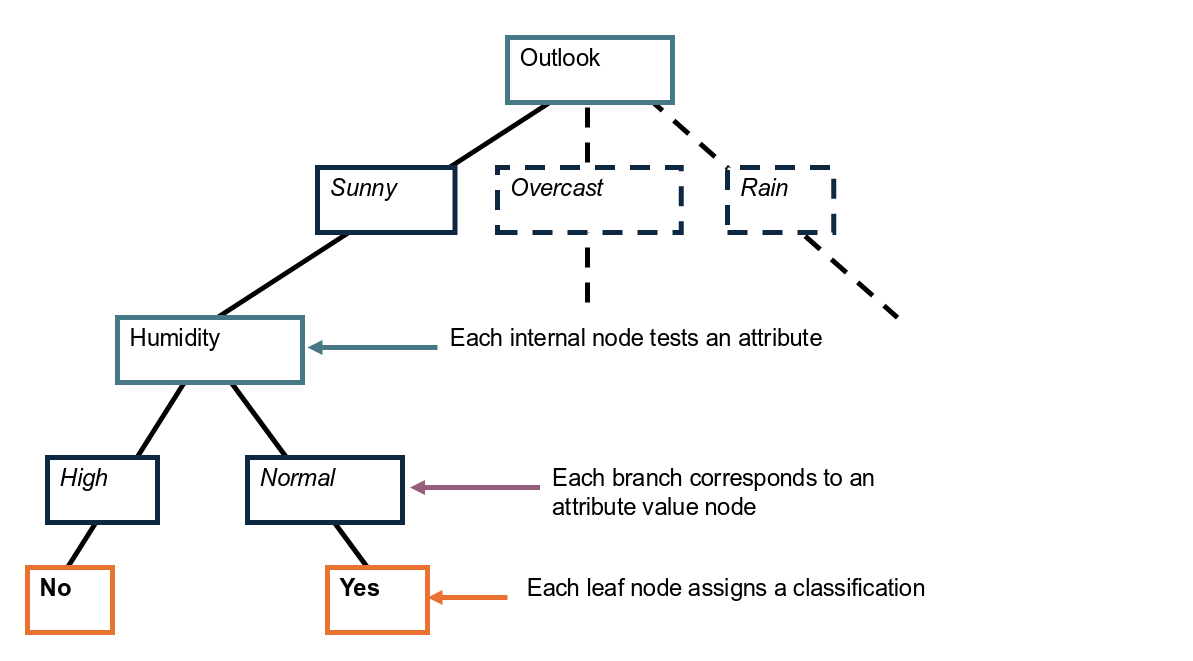
\includegraphics[width=0.8\textwidth]{pictures/decisionTree.png}
	\caption{Esempio di albero di decisione per la classificazione }
\end{figure}
Da notare che non tutti gli attributi necessariamente concorrono alla classificazione.
Gli alberi di decisione rappresentano quindi disgiunzioni di congiunzioni di condizioni sugli attributi.
Questo perché ogni cammino dalla radice a una foglia rappresenta una congiunzione di condizioni sugli attributi, l'insieme dei cammini che portano a una stessa etichetta rappresenta una disgiunzione di congiunzioni.
\\
Perché usare gli alberi di decisione?
Esplicitano la relazione tra attributi e sono facilmente interpretabili.
\\ \\
Consideriamo allora l'insieme di disgiunzioni di congiunzioni, se non ci sono esempi contraddittori allora la formula è vera per ogni esempio positivo e falsa per ogni esempio negativo,
dunque è consistente con il dataset di addestramento.
Vogliamo però inoltre che la formula sia il più piccola possibile (rimanendo valida), dato che è la nostra euristica per una buona generalizzazione.
Vogliamo trovare la formula equivalente minima.
Posso rimuovere controlli non necessari, ad esempio se ho la formula
\[
(\mathrm{Outlook}=\mathrm{Rain}) \land (\mathrm{Temperature}=\mathrm{Hot}) \land (\mathrm{Humidity}=\mathrm{High}) \land (\mathrm{Wind}=\mathrm{Weak}) \lor
\]
\[
(\mathrm{Outlook}=\mathrm{Rain}) \land (\mathrm{Temperature}=\mathrm{Hot}) \land (\mathrm{Humidity}=\mathrm{High}) \land (\mathrm{Wind}=\mathrm{Strong})
\]
dato che l'ultimo attributo non influenza il risultato (weak e strong sono tutti i possibili valori di wind) posso rimuoverlo, ottenendo
\[
(\mathrm{Outlook}=\mathrm{Rain}) \land (\mathrm{Temperature}=\mathrm{Hot}) \land (\mathrm{Humidity}=\mathrm{High}).
\]
Un altro caso è quando due o più congiunzioni contengono la stessa sottoformula, dunque non dovrebbero essere valutate nuovamente.
\\
Gli alberi di decisione dividono lo spazio delle feature in iper rettangoli con assi paralleli agli assi delle feature.
Ogni regione rettangolare viene etichettata con una classe (o una distribuzione di probabilità sulle classi).
\begin{figure}[h]
	\centering
	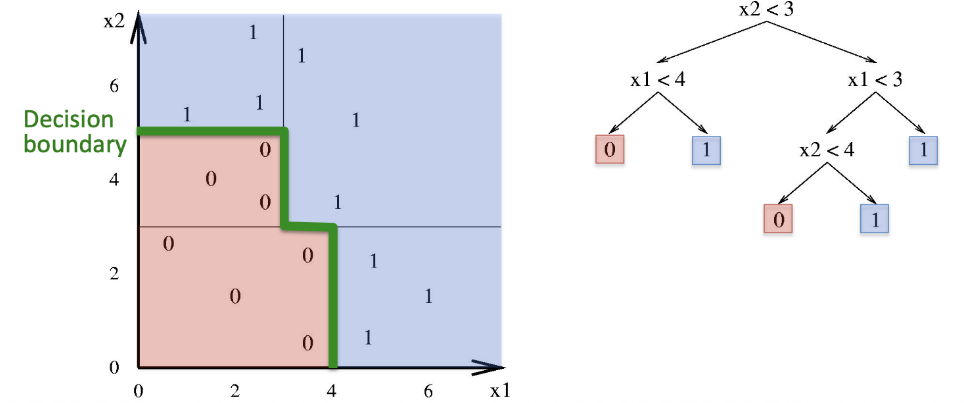
\includegraphics[width=\textwidth]{pictures/decisionBoundary.png}
	\caption{Esempio di partizionamento dello spazio delle feature tramite un albero di decisione}
\end{figure}
Questo partizionamento è chiamato \textit{decision boundary}.